\documentclass{beamer}
\setbeamertemplate{caption}[numbered]
\usetheme{Madrid}

\title[Оценивание значимости выравнивания]{Задачи оценивания значимости выравнивания при помощи скрытых марковских моделей}
\author[Власенко Даниил]{Власенко Даниил Владимирович \\ Научный руководитель: к.ф.-м.н. Коробейников А.И.\\ \vspace{1cm} Отчет по производственной практике}
\date[Декабрь 2021]{Санкт-Петербург\\Октябрь 2022}
\institute[]{Санкт-Петербургский государственный университет\\ Кафедра "Статистического моделирования"} 

\usepackage{amsmath,amssymb,amsthm,amscd,amsfonts}
\usepackage[utf8]{inputenc}
\usepackage[russian]{babel}
\usepackage{wrapfig}

\newtheorem{defenition}{Определение}

\begin{document}
	\begin{frame}
		\titlepage
	\end{frame}

	\begin{frame}{Введение}
		\begin{defenition}
			Выравнивание последовательностей  "--- размещение двух или более последовательностей друг под другом таким образом, чтобы было легче увидеть их схожие участки.
		\end{defenition}
	
		\begin{figure}
			\begin{tabular}{cccccccc}
				A&C&E&A&A&F&A&E\\
				C&E&A&F&D&C&E&\\
			\end{tabular}
		\end{figure}
		\begin{figure}
			\begin{tabular}{ccccccccc}
				A&C&E&A&A&F&A&—&E\\
				—&C&E&A&—&F&D&C&E\\
			\end{tabular}
			\caption{Последовательности до и после выравнивания.} \label{fg:1}
		\end{figure}
	
		\begin{defenition}
			Значимость выравнивания "--- действительное число $s$, отражающее сходство последовательностей.
		\end{defenition}
	\end{frame}

	\begin{frame}{Введение}
		\begin{itemize}
			\item достаточно ли высокая значимость, чтобы считать последовательность не шумом, или шум мог добиться такой значимости.
			\item достаточно ли низкая значимость, чтобы считать последовательность шумом, или не шум мог получить такую значимость. 
		\end{itemize}
	
		\begin{defenition}
			Ложноположительная вероятность значимости $s$ "--- это вероятность того, что шум получит значимость равную или выше $s$. 
		\end{defenition}
	\end{frame}

	\begin{frame}{Обозначения и известные результаты}
		\begin{defenition}
			Пусть $X_{n}$ и $Y_{n}$ дискретные стохастические процессы, $n \geq 1$. Пара $(X_{n}, Y_{n})$ называется скрытой марковской моделью, если
			\begin{itemize}
				\item $X_{n}$~--- марковский процесс, поведение которого напрямую не наблюдается ("скрытый");
				\item $\mathsf{P}(Y_{n} = y_{n}|X_{1} = x_{1},\dots, X_{n} = x_{n}) = \mathsf{P}(Y_{n}|X_{n}=x_{n})$ для любого $n \geq 1$, где $x_{1},\dots,x_{n}$~--- значения, принимаемые процессом  $X_{n}$ (\textbf{состояния модели}), $ y_{n}$~--- значение, принимаемое процессом $Y_{n}$ (\textbf{наблюдаемый символ модели}).
			\end{itemize}
		\end{defenition}		
	\end{frame}

	\begin{frame}{Обозначения и известные результаты}
		\begin{figure}[h]
			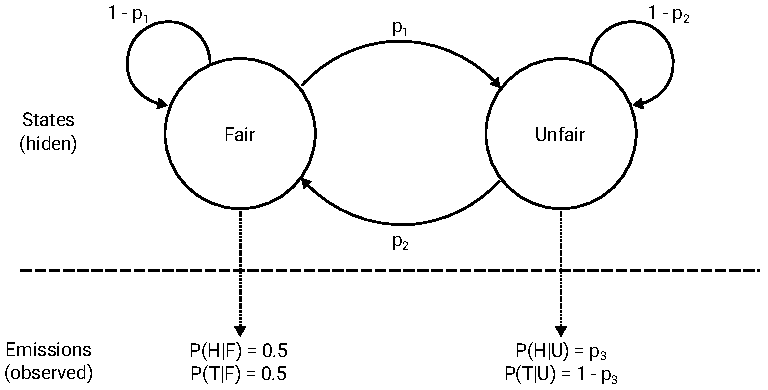
\includegraphics[width=10cm]{../report/figure1}
			\caption{Простая скрытая марковская модель.} \label{fg:2}
		\end{figure}
	\end{frame}

	\begin{frame}{Обозначения и известные результаты}
		\begin{figure}[h]
			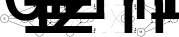
\includegraphics[width=12cm]{../report/figure2}
			\caption{Профильная скрытая марковская модель.}  \label{fg:3}
		\end{figure}		
	\end{frame}

	\begin{frame}{Обозначения и известные результаты}
		\begin{defenition}
			\textit{Вероятность последовательности} $D$ может интерпретироваться и считаться по-разному "--- алгоритмом \textit{Витерби} или \textit{Форвард} алгоритмом.
		\end{defenition}
		
		\begin{equation*}
			s_{max}(D) = \underset{\pi \in \pi_{D}}{max}(s(\pi)); \label{eq:1}
		\end{equation*}
	
		\begin{equation*}
			s_{fw}(D) = \sum_{\pi \in \pi_{D}}s(\pi); \label{eq:2}
		\end{equation*}
	
		\begin{equation*}
			Z(D, T)	= \sum_{\pi \in \pi_{D}}s(\pi)^{\frac{1}{T}}. \label{eq:3}
		\end{equation*}
	\end{frame}	

	\begin{frame}{Обозначения и известные результаты}
		Мы предполагаем наличие простой фоновой модели $B$ для последовательностей длины $L$ такой, что все $L$ символьных позиций независимы и одинаково распределены в соответствии с некоторым распределением $\mathsf{P}(d|B)$, где $d$ отражает возможный наблюдаемый символ:
		\begin{equation*}
			\mathsf{P}(D|B) = \prod_{i=1}^{L}\mathsf{P}(d_{i}|B), \label{eq:4}
		\end{equation*}
		где $d_{i}$ "--- это $i$-ый наблюдаемый символ последовательности $D$.
	\end{frame}

	\begin{frame}{Обозначения и известные результаты}
		\begin{defenition}
			Ложноположительная вероятность значимости $s_{0}$ для строк длины $L$:	
			\begin{equation}
				fpr(s_{0}) =  \sum_{D \in D_{L}} \mathsf{P}(D|B) \Theta(s(D) \geq s_{0}), \label{eq:5}
			\end{equation}
			где $\mathsf{P}(D|B)$ "--- условная вероятность последовательности $D$, описываемая фоновой моделью, $s(D)$ "--- вероятность последовательности $D$, считаемая профильной СММ, и
			\[
			\Theta(s(D) \geq s_{0}) = 
			\begin{cases}
				1, & s(D) \geq s_{0}\\
				0, & s(D) < s_{0}
			\end{cases}.
			\]
		\end{defenition}		
	\end{frame}
	
	\begin{frame}{Обозначения и известные результаты}
		Вычисление $fpr(s_{0})$ через формулу \eqref{eq:5} обычно неосуществимо, значение $fpr(s_{0})$ может быть оценено через выборку по значимости. 
		
		\vspace{0.5cm}
		
		Пусть $\mathsf{P}(D|T)$ "--- это условная вероятность строки $D$ относительно некоторой модели строк длины $L$ параметризованной значением $T$. Тогда можно переписать $fpr(s_{0})$:		
		
		\begin{equation*}
			fpr(s_{0}) = \sum_{D \in D_{L}} \mathsf{P}(D|T) f(D,s_{0}), \label{eq:6}
		\end{equation*}
		где
		\begin{equation}
			f(D,s_{0}) = \frac{\mathsf{P}(D|B) \Theta(s(D) \geq s_{0})}{\mathsf{P}(D|T)}. \label{eq:7}
		\end{equation}				
	\end{frame}

	\begin{frame}{Обозначения и известные результаты}
		Определим модель, используемую для выборки по важности параметризованную $T$:		
		
		\begin{equation*}
			\mathsf{P}(D|T) = \frac{\mathsf{P}(D|B)Z(D,T)}{Z(T)}, \label{eq:8}
		\end{equation*}							
		где 
		\begin{equation*}
			Z(T) = \sum_{D \in D_{L}}\mathsf{P}(D|B)Z(D,T). \label{eq:9}
		\end{equation*}
		Подставив определение $\mathsf{P}(D,T)$ в уравнение \eqref{eq:7} получим
		\begin{equation*}
			f(D,s_{0}) = \frac{Z(T)\Theta(s(D) \geq s_{0})}{Z(D,T)}. \label{eq:10}
		\end{equation*}	
	\end{frame}

	\begin{frame}{Полученные результаты}
		Вычислим оценку $\widehat{fpr}(s_{0})$ для строк длины $L=100$, состоящих из 5 символов, и доверительные интервалы уровня $\gamma = 0.99$:		
		\begin{table}
			\caption{Результаты} \label{tb:1}
			\begin{tabular}{cccc}
				$s_{0}$&T&$\widehat{fpr}(s_{0})$&$[c_{1}(\gamma);c_{2}(\gamma)]$  \\ \hline
				$10^{-85}$&7&0.0000000183&[0.0; 0.00066349] \\
				$10^{-90}$&7&0.003175&[0.001884; 0.004779] \\ 
				$10^{-100}$&7&0.615709&[0.597540 0.622677] \\
			\end{tabular}
		\end{table}								
	\end{frame}

	\begin{frame}{Заключение}
		\begin{itemize}
			\item Была изучена тема алгоритмов парного и множественного выравнивания последовательностей и тема СММ и алгоритмов взаимодействия с ними.
			\item Был реализован алгоритм, позволяющий эффективно вычислять оценку ${fpr}(s_{0})$.
			\item Предстоит подробно верифицировать реализованный алгоритм и сравнить его с имеющимися методами вычисления оценки ${fpr}(s_{0})$.
		\end{itemize}
	\end{frame}

	\begin{frame}{Список литературы}
		\nocite{Newberg2009}
		\nocite{Compeau2015}
		\nocite{Compeau2015a}
		\nocite{Dugad1996}		
		\bibliographystyle{../report/ugost2008mod}
		\bibliography{../report/references}
	\end{frame}


\end{document}